% -*-latex-*-
% 
% For questions, comments, concerns or complaints:
% thesis@mit.edu
% 
%
% $Log: cover.tex,v $
% Revision 1.8  2008/05/13 15:02:15  jdreed
% Degree month is June, not May.  Added note about prevdegrees.
% Arthur Smith's title updated
%
% Revision 1.7  2001/02/08 18:53:16  boojum
% changed some \newpages to \cleardoublepages
%
% Revision 1.6  1999/10/21 14:49:31  boojum
% changed comment referring to documentstyle
%
% Revision 1.5  1999/10/21 14:39:04  boojum
% *** empty log message ***
%
% Revision 1.4  1997/04/18  17:54:10  othomas
% added page numbers on abstract and cover, and made 1 abstract
% page the default rather than 2.  (anne hunter tells me this
% is the new institute standard.)
%
% Revision 1.4  1997/04/18  17:54:10  othomas
% added page numbers on abstract and cover, and made 1 abstract
% page the default rather than 2.  (anne hunter tells me this
% is the new institute standard.)
%
% Revision 1.3  93/05/17  17:06:29  starflt
% Added acknowledgements section (suggested by tompalka)
% 
% Revision 1.2  92/04/22  13:13:13  epeisach
% Fixes for 1991 course 6 requirements
% Phrase "and to grant others the right to do so" has been added to 
% permission clause
% Second copy of abstract is not counted as separate pages so numbering works
% out
% 
% Revision 1.1  92/04/22  13:08:20  epeisach

% NOTE:
% These templates make an effort to conform to the MIT Thesis specifications,
% however the specifications can change.  We recommend that you verify the
% layout of your title page with your thesis advisor and/or the MIT 
% Libraries before printing your final copy.
\title{RNA Macrostates and Computational Tools}

\author{Michael Flynn}
% If you wish to list your previous degrees on the cover page, use the 
% previous degrees command:
%       \prevdegrees{A.A., Harvard University (1985)}
% You can use the \\ command to list multiple previous degrees
%       \prevdegrees{B.S., University of California (1978) \\
%                    S.M., Massachusetts Institute of Technology (1981)}
\department{Department of Phyiscs}

% If the thesis is for two degrees simultaneously, list them both
% separated by \and like this:
% \degree{Doctor of Philosophy \and Master of Science}
\degree{Bachelors of Art in Physics}

% As of the 2007-08 academic year, valid degree months are September, 
% February, or June.  The default is June.
\degreemonth{June}
\degreeyear{2015}
\thesisdate{May 18, 2015}

%% By default, the thesis will be copyrighted to MIT.  If you need to copyright
%% the thesis to yourself, just specify the `vi' documentclass option.  If for
%% some reason you want to exactly specify the copyright notice text, you can
%% use the \copyrightnoticetext command.  
%\copyrightnoticetext{\copyright IBM, 1990.  Do not open till Xmas.}

% If there is more than one supervisor, use the \supervisor command
% once for each.
\supervisor{Daniel Aalberts}{Professor of Physics}

% This is the department committee chairman, not the thesis committee
% chairman.  You should replace this with your Department's Committee
% Chairman.
\chairman{Arthur C. Smith}{Chairman, Department Committee on Graduate Theses}

% Make the titlepage based on the above information.  If you need
% something special and can't use the standard form, you can specify
% the exact text of the titlepage yourself.  Put it in a titlepage
% environment and leave blank lines where you want vertical space.
% The spaces will be adjusted to fill the entire page.  The dotted
% lines for the signatures are made with the \signature command.
\maketitle 

% The abstractpage environment sets up everything on the page except
% the text itself.  The title and other header material are put at the
% top of the page, and the supervisors are listed at the bottom.  A
% new page is begun both before and after.  Of course, an abstract may
% be more than one page itself.  If you need more control over the
% format of the page, you can use the abstract environment, which puts
% the word "Abstract" at the beginning and single spaces its text.

%% You can either \input (*not* \include) your abstract file, or you can put
%% the text of the abstract directly between the \begin{abstractpage} and
%% \end{abstractpage} commands.

% First copy: start a new page, and save the page number.
\cleardoublepage
% Uncomment the next line if you do NOT want a page number on your
% abstract and acknowledgments pages.
% \pagestyle{empty}
\setcounter{savepage}{\thepage}
%\begin{abstractpage}
%% $Log: abstract.tex,v $
% Revision 1.1  93/05/14  14:56:25  starflt
% Initial revision
% 
% Revision 1.1  90/05/04  10:41:01  lwvanels
% Initial revision
% 
%
%% The text of your abstract and nothing else (other than comments) goes here.
%% It will be single-spaced and the rest of the text that is supposed to go on
%% the abstract page will be generated by the abstractpage environment.  This
%% file should be \input (not \include 'd) from cover.tex.
In this thesis, I designed and implemented a compiler which performs
optimizations that reduce the number of low-level floating point operations
necessary for a specific task; this involves the optimization of chains of
floating point operations as well as the implementation of a ``fixed'' point
data type that allows some floating point operations to simulated with integer
arithmetic.  The source language of the compiler is a subset of C, and the
destination language is assembly language for a micro-floating point CPU.  An
instruction-level simulator of the CPU was written to allow testing of the
code.  A series of test pieces of codes was compiled, both with and without
optimization, to determine how effective these optimizations were.

%\end{abstractpage}

% Additional copy: start a new page, and reset the page number.  This way,
% the second copy of the abstract is not counted as separate pages.
% Uncomment the next 6 lines if you need two copies of the abstract
% page.
% \setcounter{page}{\thesavepage}
% \begin{abstractpage}
% % $Log: abstract.tex,v $
% Revision 1.1  93/05/14  14:56:25  starflt
% Initial revision
% 
% Revision 1.1  90/05/04  10:41:01  lwvanels
% Initial revision
% 
%
%% The text of your abstract and nothing else (other than comments) goes here.
%% It will be single-spaced and the rest of the text that is supposed to go on
%% the abstract page will be generated by the abstractpage environment.  This
%% file should be \input (not \include 'd) from cover.tex.
In this thesis, I designed and implemented a compiler which performs
optimizations that reduce the number of low-level floating point operations
necessary for a specific task; this involves the optimization of chains of
floating point operations as well as the implementation of a ``fixed'' point
data type that allows some floating point operations to simulated with integer
arithmetic.  The source language of the compiler is a subset of C, and the
destination language is assembly language for a micro-floating point CPU.  An
instruction-level simulator of the CPU was written to allow testing of the
code.  A series of test pieces of codes was compiled, both with and without
optimization, to determine how effective these optimizations were.

% \end{abstractpage}



\section*{Acknowledgments}

I owe gratitude to a great many people. Thank you to my thesis advisor
Daniel Aalberts for accepting me as your thesis student and advising
me through the long process of writing a thesis. With your help and
encouragement I felt like I was able to make an impact in the field as
an undergraduate. I'd like to thank the faculty of the Physics
department of Williams College who have instructed me including Bill
Wootters, Kevin Jones, David Tucker-Smith, Ward Lopes, Michael
Seifert, Frederick Strauch, and Charlie Doret for their patience,
support and incredibly lucid explanations. I'd also like to thank the
Computer Science faculty, including Tom Murtagh, Jeannie Albrect,
Brent Heeringa, Morgan McGuire, Duane Bailey, Bill Lenhart, Stephen
Freund, and Brent Yorgey for their patience as well, and for making
some of my favorite classes at Williams.

I'd like to thank Michael Zuker and David Mathews for their
correspondence and help getting started in the field of RNA secondary
structure research. Thank you to Nick Markham for writing a very clear
Ph. D. thesis. 

I'd like to thank my friends including Maoli Vizcaino for keeping me
company while I toil, Tony Blanco, Qadir Forbes, JL Etienne and Dan
Evangelakos for their support, good conversations, and friendship. 

Most of all I'd like to thank my parents Michell and James Flynn and the rest of my family Matt, Emma, Daniel, Genny, Elizabeth, Marie, Elise, and Lily for always
being there. No matter happens, I know I can come home to open arms.

\newpage

\section*{Executive Summary}

RNA is a biological polymer built from monomers that can form
basepairs with each other. There are a multitude of possible folds,
including many local free energy minima. Computational tools exist for
finding the minimum free energy state (MFE) and computing the
probability for a given pair from the partition function. A
significant motivation for this thesis is the current movement away
from looking at RNA as a molecule with a single folding determined by
the MFE state to looking at RNA as a system in equilibrium between
several different macrostates with possibly degenerate free
energies. Macrostates can be defined as a set of foldings sufficiently
close to a local minimum.

This thesis describes several tools to build macrostates and compute
their partition functions. In the process we also improve upon the
partition function and stochastic traceback algorithms. These
algorithmic improvements restructure the computations into equivalent
formulations where each base iterates over a list of other bases it
can pair to. By default, we can assume nothing and check every case,
like the current algorithm does, but restricting the allowed pairs for
a base can eliminate large amounts of unnecessary computation. This is
very reasonable in practice, as Figure \ref{fig:probThresh1} shows.
To restrict to probable pairs introduces minimal error, but is an
order of magnitude faster. The most significant results of this thesis
are the derivation of these new formulations and their
implementations. By eliminating pairs below a reasonable probability
threshold like $\theta = 10^{-8}$, massive speedups can be seen that
cost very small amounts of error as illustrated by Figures
\ref{fig:pfResults1} and \ref{fig:stochOvN1}.

Other results of this thesis include an algorithm to predict
macrostates (NestorPF) and a method of clustering analysis on SHAPE
reactivity data in mutate-and-map experiments. NestorPF uses a measure
called non-nestedness to split ensembles recursively. The SHAPE data
analysis is important because, unlike most experimental procedures in
RNA structure determinations, SHAPE reactivity provides a softer
constraint on structure where the strength of a signal can be
interpreted as a probability instead of as a determined pair or not. 

\begin{figure}[t]
\centering
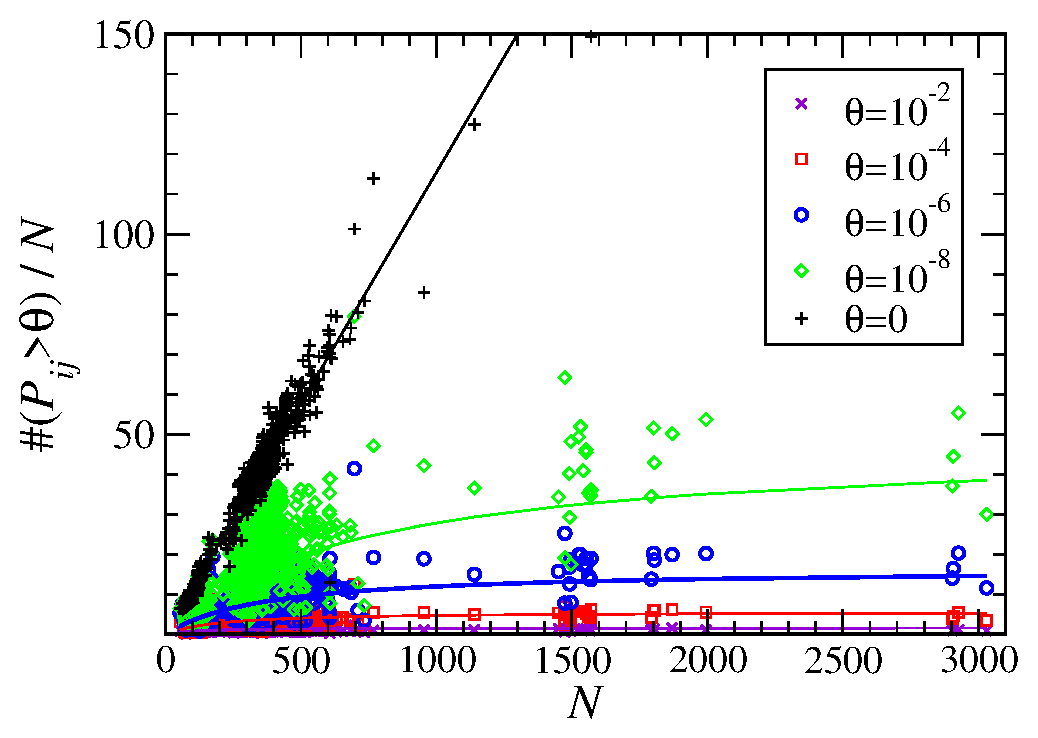
\includegraphics[width=.8\textwidth]{PijTheta5.eps} 
\caption[Number of probable pairs above threshold $\theta$]{A plot of
  `number of pairs with probability greater than colored threshold
  vs length of sequence. If there is no threshold, the number of pairs
  possible goes up like $n^2$, but even with small thresholds such as
  requiring a pair to have probability greater than $10^{-8}$, the
  number of possible pairs goes flat as $n$ increases. Therefore, a
  great amount of efficiency can be gained by restricting the pairs
  under consideration, while not sacrificing much accuracy since the
  thresholds are so low. }
\label{fig:probThresh1}
\end{figure}
\begin{figure}[t]
\centering
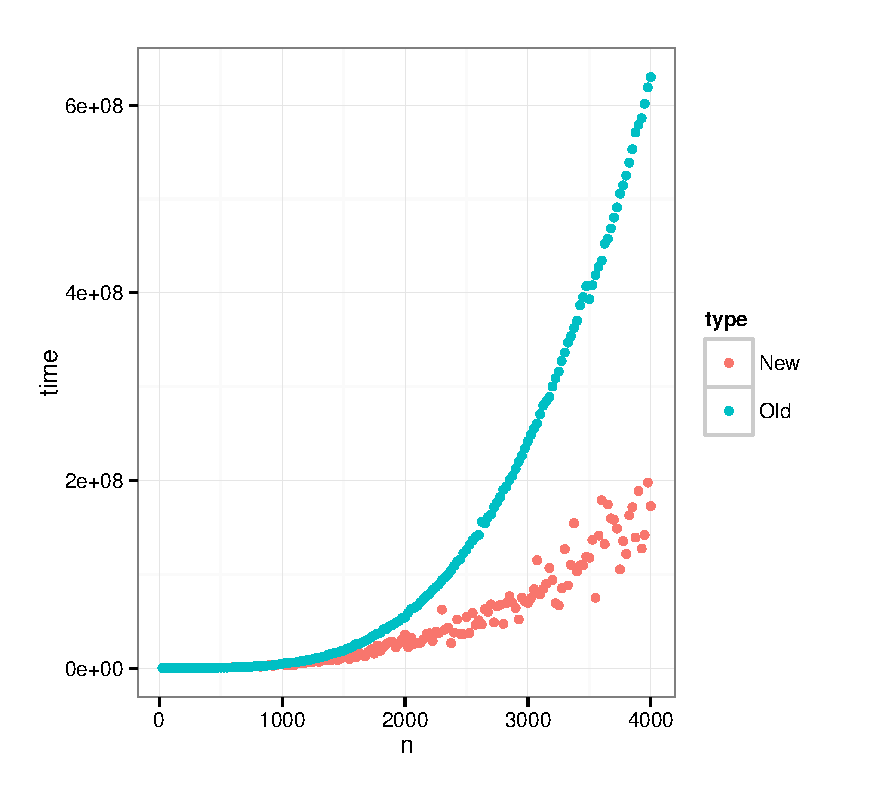
\includegraphics[width=.75\textwidth]{partitionTimePlot.eps} 
\caption[Partition Function Speedups]{Computation time vs length for
  random sequences, the old $O(n^3)$ partition function run against
  the new $O(n^2)$ partition function. Not quite the results we were
  after, however, we can always set the max internal loop length $L$
  to a lower value and increase the probability threshold $\theta$.}
\label{fig:pfResults1}
\end{figure}
\begin{figure}[t]
\centering
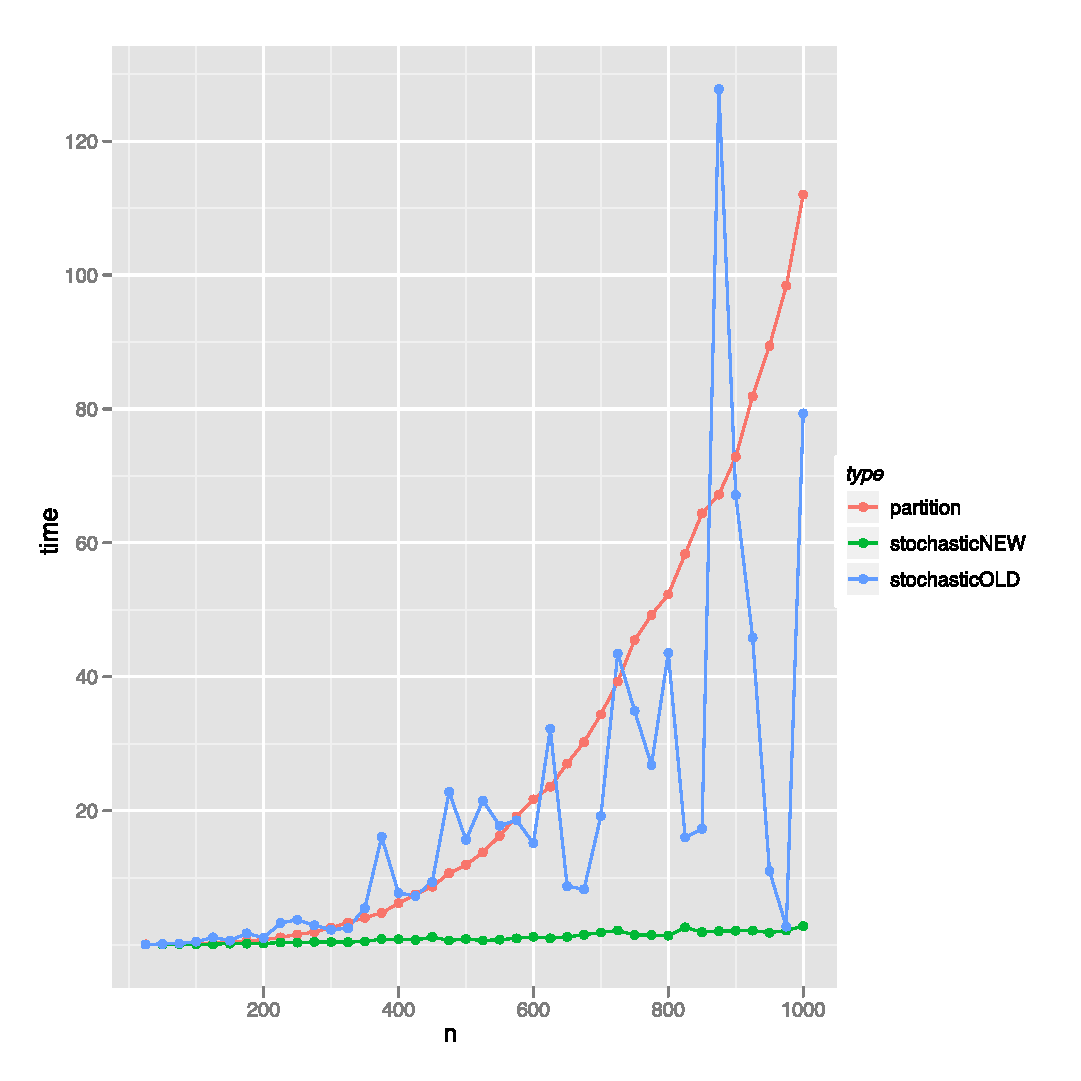
\includegraphics[width=.75\textwidth]{stochOldvNew.eps}
\caption[Stochastic Traceback Speedups]{A comparison of the
  computation time between the partition function computation, and
  stochastic tracebacks of 1000 samples with the Old algorithm and the
  new algorithm. The new algorithm is much faster.}
\label{fig:stochOvN1}
\end{figure}
\begin{figure}[t]
\centering
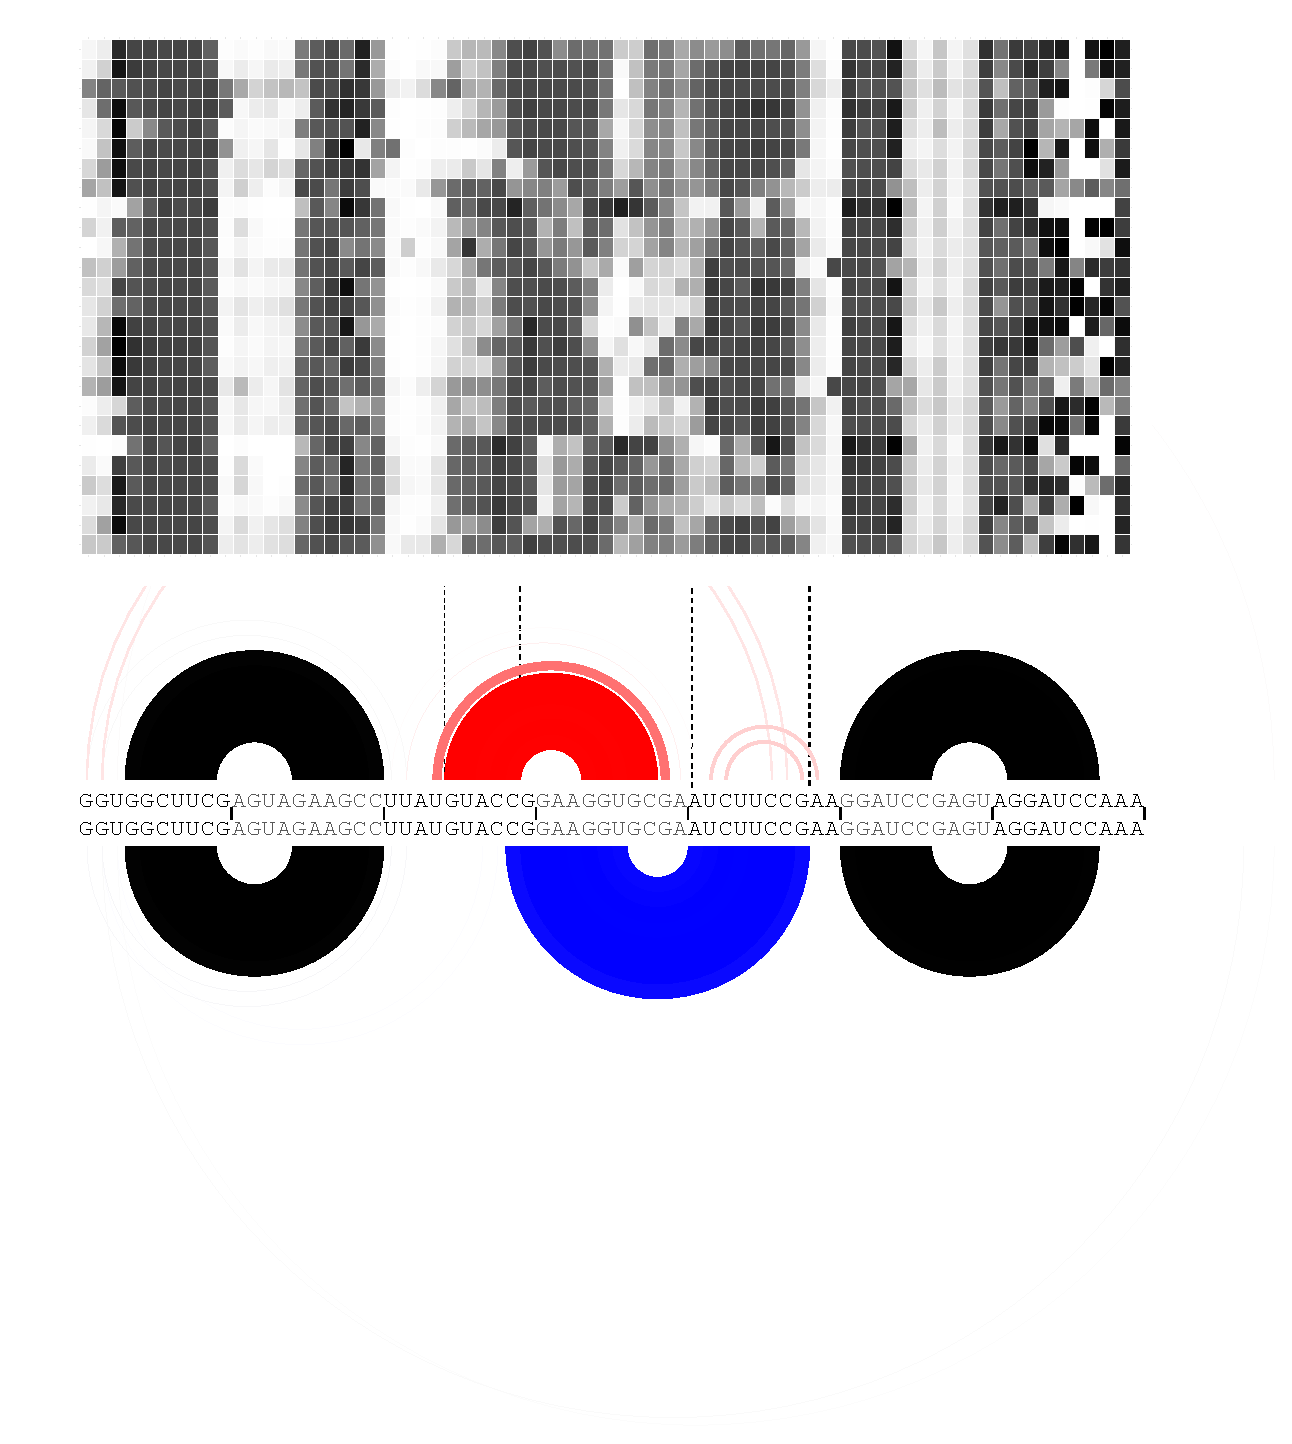
\includegraphics[width=\textwidth]{Nestor-Heatmap-agreement.eps}
\caption[Nestor-Reactivity Agreement]{ Mutate-and-map experimental
  results are plotted on top of an RNAbow. In places where the
  dominant blue cluster is disrupted, the red cluster becomes
  dominant. The alignment of the stems with the dark lines on the
  heatmap show agreement between Nestor and experiment.}
\label{fig:Nestor-Heatmap-agreement}
\end{figure}
In Chapter 1, I describe the RNA free energy model and its
implementation in classic RNA folding algorithms. The model is large,
complex, and important to understand in order to understand the
algorithms in later chapters.

Chapter 2 presents the algorithm to compute the partition function of
RNA and my improvements to that algorithm. I show that with an allowed
base-pairs heuristic, we can significantly speed up the computation.

Chapter 3 presents the algorithm for sampling secondary structures
according to the Boltzmann ensemble, called the stochastic traceback
algorithm, and my improvements to that algorithm. These improvements
mirror those in chapter 2.

Chapter 4 defines macrostates and examines previous methods of
grouping structures including Ding and Lawrence's Sfold, Barriers from
ViennaRNA, and Nestor from Aalberts and Jannen. I then present a new
approach to Nestor, splitting clusters based on partition function
results, which I call NestorPF. Finally I describe SHAPE chemical
mapping experiments to probe RNA structure, our method to process
mutate-and-map experimental data. We compare our analysis of
mutate-and-map experiments with NestorPF prediction.

Chapter 5 concludes and presents some future work, including the
prospects of using the known-pairs heuristic to create a pseudoknot
algorithm, which could greatly expand the predictive ability of RNA
secondary structures.


%%%%%%%%%%%%%%%%%%%%%%%%%%%%%%%%%%%%%%%%%%%%%%%%%%%%%%%%%%%%%%%%%%%%%%
% -*-latex-*-
